\chapter{Fundamentação teórica}
\label{cap:fundamentacao-teorica}

Neste capítulo, a fundamentação teórica das tecnologias abordadas neste trabalho é realizada. Conceitos básicos sobre a linguagem de programação Java são mostrados, abordando tanto os pilares da orientação a objetos presente na linguagem quanto bibliotecas relevantes para as aplicações desenvolvidas na área. Posteriormente, conceitos relevantes para a o desenvolvimento de interfaces de usuário (\textit{user interface}, UI) e experiência de usuário (\textit{user experience}, UX) são apresentados, apontando características e ferramentas utilizada no processo de construção de interfaces.

\section{Java}
\label{sec:java}

Uma das tecnologias presentes no Programa de Estágio Jedi Internship e abordadas nesse trabalho corresponde ao aprendizado e aplicação de conceitos da linguagem de programação Java. Originada inicialmente em 1991 com o codinome de Oak, e nomeada de Java somente em 1995, atualmente a linguagem é uma das mais utilizadas na área de Computação, sendo administrada pela empresa Oracle e estando em sua oitava versão~\cite{ocastudyguide-2015}.

Em suas primeiras versões, o propósito inicial do Java era conectar diferentes tipos de micro-sistemas da empresa Sun, sendo uma linguagem comum entre eles. A habilidade de escrever um código que pode funcionar em mais de um sistema é conhecida como \textit{write once, run anywhere} (WORA), sendo uma das principais características da linguagem. Ao escrever um código em Java, o compilador Javac processa o arquivo fonte para um arquivo em \textit{bytecode}, e um interprador JVM específico para a plataforma se encarrega de processar essearquivo posteriormente, como mostrado na Figura~\ref{fig:java-fluxo}~\cite{ocastudyguide-2015}.

\begin{figure}[htb!]
  \centering
  \caption{Esquema de execução de um código escrito em Java}
  \label{fig:java-fluxo}
  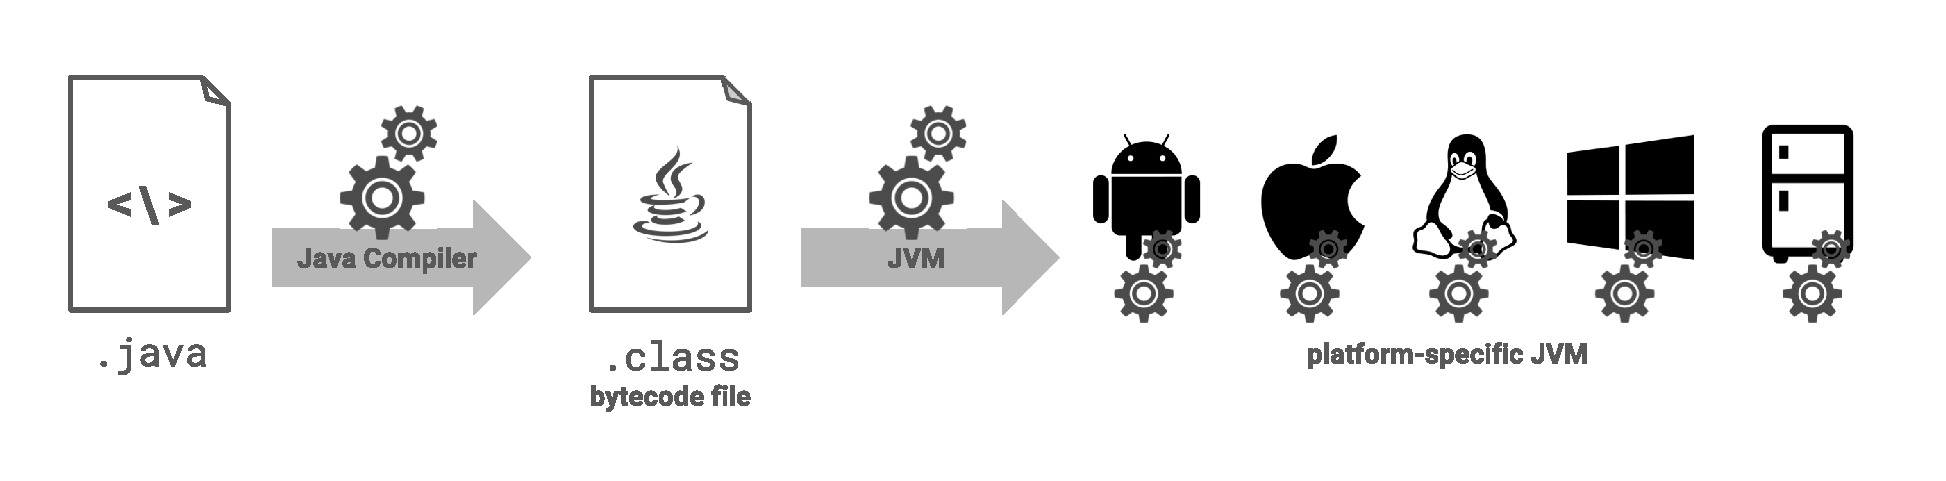
\includegraphics[width=\textwidth, keepaspectratio=true]{img/java-fluxo}
  \fonte{Próprio autor.}
\end{figure}

Além do WORA, outra característica marcante da linguagem é a implementação do conceito de orientação a objetos. Para implementar tal conceito, o Java faz uso de classes e objetos: enquanto uma classe funciona como uma especificação de uma ideia, um objeto corresponde a uma instância, uma materialização dessa ideia, sendo que uma classe pode possuir vários objetos instanciados~\cite{ocastudyguide-2015}.

A relação entre classes e objetos dá margem para diversos outros conceitos presentes na linguagem Java. O conceito de encapsulamento, por exemplo, faz uso de modificares de acesso nos atributos e métodos de cada classe para controlar quais objetos podem acessá-los, enquanto o conceito de herança entre as classes determina uma relação de pai-filho entre elas, tornando possível que uma herde atributos e métodos da outra~\cite{ocastudyguide-2015}.

Conceitos de abstração, composição e interfaces também estão presentes na linguagem, possibilitando a criação de classes não instanciáveis, classes compostas por diversos objetos, e a garantia que alguns métodos são implementados em determinadas classes, respectivamente. Por fim, um conceito essencial da linguagem é o polimorfismo, que permite que um objeto seja referenciado por diversas maneiras, como por meio das classes que ele herda, ou de interfaces que implementa~\cite{ocastudyguide-2015}.

Além dos conceitos apresentados, o Java ainda conta com bibliotecas como o \textit{collections framework}, que implementam diferentes estruturas de dados utilizadas comumente na programação de computadores. Estruturas como \textit{hashes}, listas de vetores, pilhas e filas podem ser utilizadas através das interfaces \verb|HashSet|, \verb|ArrayList|, \verb|Stack| e \verb|Queue|, respectivamente. Além de eliminar a necessidade do programador construir cada uma das estruturas, a utilização delas é extremamente comum em aplicações construídas em Java, facilitando o trabalho do desenvolvedor~\cite{javacollections-2001}.

Tanto os elementos presentes no \textit{collections framework} quanto os conceitos apresentados previamente podem ser utilizados para diversos tipos de aplicações em Java~\cite{javacollections-2001}. O gerenciamento de banco de dados relacionais em Java, por exemplo, utiliza uma interface de programação de aplicações (\textit{application programming interface}, API) chamada Java Database Connectivity (JDBC). O JDBC abstrai a implementação de banco de dados específicos, criando uma camada única que contribui para a implementação de métodos para estabelecer conexões, criar \textit{queries} de acesso, e extrair resultados de buscas, por exemplo~\cite{databaseprogramming-2000}.

O JDBC ainda conta com maneiras para gerenciar múltiplas conexões em um servidor através de um \textit{pool} de conexões, e de centralizar o acesso de dados por meio de objetos de acesso a dados (\textit{data access object}, DAO)~\cite{databaseprogramming-2000}. A utilizadação de alguns desses recursos é aprofundada na Seção~\ref{sec:java-atividades} do Capítulo~\ref{cap:atividades-desenvolvidas}, que descreve as atividades realizadas durante a área de Java do Programa de Estágio.

\section{\textit{User interface} e \textit{user experience}}
\label{sec:user-interface-e-user-experience}

A ser escrita.
